\documentclass[main.tex]{subfiles}
\begin{document}
  \section{The Model}
    
    The model was implemented in Mathematica 11.3 \cite{wolfram}, and can be viewed at: \url{https://github.com/SonkeWohler/PX4514}.
    
    \subsection{Fundamental Model Structure}
      
      The playing field within the model is represented as a coordinate system as shown in \Cref{fig:field}. Over these coordinates each position has a number of properties detailed in \Cref{tab:positions}. These positions are used to refer to the players independent of their coordinates. \\
      Position 0 refers to the setter independent of their position within the rotation. For example, \(x_{0,current}\) refers to the x coordinate of the current setter position.
      \\\\
      The model uses this coordinate system to calculate distances, like the \(distance_{setter \to ideal}\) defined in \Cref{equ:distIdeal} i.e. the distance between the setter's current  position and the ideal setter coordinates. \\
      The ideal setter coordinates (see \Cref{tab:positions} Setter) describe the point from which the setter has the most freedom because they can reach the ball comfortably, making it easy to set, and from this point they can reach almost any position easily. This is the point on the field that the setter always attempts to reach \cite{idealSetter}. \\
      Being further away from this position reduces the setter's ability to choose a good set, and forces them to set to the few positions they can actually reach.\\
      This difficulty is represented by \Cref{equ:easeSet}, which describes how easily the setter can set to a position of their choice.
      
      \begin{subequations}
       \begin{equation}
        distance_{max} = 8 \sqrt{2}
        \label{equ:distMax}
       \end{equation}
       \begin{equation}
         distance_{setter \to Ideal} = \sqrt{|x_{0,current} - x_{0,ideal}|^2 + 
         |y_{0,current} - y_{0,ideal}|^2}
         \label{equ:distIdeal}
        \end{equation}
        \begin{equation}
          ease_{Setting} = 1 - \frac{distance_{setter \to Ideal}}{distance_{max}}
          \label{equ:easeSet}
        \end{equation}
        \label{equ:dist}
      \end{subequations} 
      
      The model also keeps track of the game score in \Cref{equ:score}, in order to add pressure to the setter's decision. The idea is that, as pressure rises, players tend to experiment less and stick to plays known to work better.
    
      \begin{subequations}
        \begin{equation}
          points_{Factor}=(points_{their} - points_{own})\frac{points_{higher}}{25} 
          \label{equ:points}
        \end{equation}
        \begin{equation}
          pressure= max( point_{Factor}, 0) + 1      
          \label{equ:pressure}
        \end{equation}
        \label{equ:score}
      \end{subequations}
      
      These quantities are used in \Cref{equ:finalPosition} to increase or decrease how e=relevant the second term is, which is affected by the difficulty of the attack from that posiition.
      
      \begin{SCfigure}
        \centering
        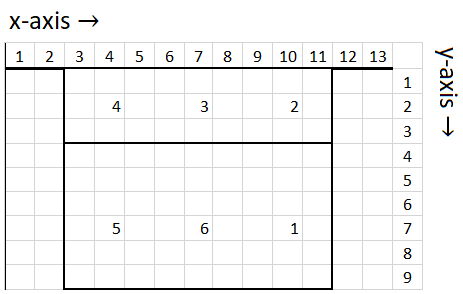
\includegraphics[width=0.5\linewidth]{figures/playingFieldGridLabelled}
        \caption{The coordinate system laid over the playing field. The net is spun at y=0 in the figure. \\
          This system is primarily used to allow the model to take player positions into account, like the distance that the setter must cover to reach the ball from their position. \\
          It is also used when noting down real world data to a format that the model can interpret.}
        \label{fig:field}
      \end{SCfigure}
    
      \begin{table}[h!]
        \centering
        \caption{Basic constants defined for each position. \\
          Each position is assigned a number of constants that help calculate parameters that are in turn used to score the different positions. \\
          Note that Position 0 either refers to the setter's coordinates or to a "Dump", an attack by the setter without first setting to another player. \\
          \textbf{Ideal Contact Coordinates} describe where a player or the setter would be if they contact the ball in the ideal position. While the setter may not always be in this position, it is assumed for the model that all other players are in their ideal position when the setter makes their decision. \\
          \textbf{Ease of Attack} (also bias or \(ease_{attack}\)) is used to tune the model. It was observed for example that positions closer to the net are more likely to be set to, as they are easier to attack from successfully. \\
          \textbf{Validity} Describes when the setter is allowed to set to a position. For example, position 5 is occupied by the Libero, a player that only defends and never attacks. 
        }
        \small
        \begin{tabular}{ c | c c c }
          \hline
          Position  & Ideal Contact Coordinates & Ease of Attack & Validity \\ \hline \hline
          Setter/Dump (0) &  8,1 & 10\% & setter y=1 \\
          1 & 10,3 & 50\% & setter is front court \\
          2 & 11,1 & 90\% & setter is back court \\
          3 & 7,1 & 70\% &  always \\
          4 & 3,1 & 90\% & always \\
          5 & invalid & invalid & never\\
          6 & 7,3 & 40\% & always \\
          \hline 
        \end{tabular}
        \label{tab:positions}
        \normalsize
      \end{table}
      
    \subsection{Scoring Positions}
      
      Ultimately the System scores each position by how likely the setter is to score to it, based on a number of factors defined in \Cref{equ:finalPosition}.\\
      Firstly, invalid positions are scored as 0 by default, see \Cref{equ:validPosition}. \\
      Furthermore, the score for each position is affected by two terms, a setter term and an attacker term. The setter term is simply the distance between that player and the setter, as defined in \Cref{equ:setPosition}. \\
      The attacker term is currently defined by \(ease_{attack}\) in \Cref{tab:positions}, but scaled by \Cref{equ:easeSet} and \Cref{equ:pressure}. As a result higher pressures or more difficult setting conditions reduce the relevance of the attacker term, and allow the setter to focus on setting to positions that they can still do so successfully, with minimal time for the opponent to react and minimal chances of mistakes \cite{idealSetter}.
      
      \begin{subequations}
        \begin{equation}
        valid_{(p)}=\left\{  
        \begin{array}{lr} 
        1 : \text{position \emph{p} is valid,  see \Cref{tab:positions}} \\
        0 : \text{otherwise}
        \end{array}
        \right.
        \label{equ:validPosition}
        \end{equation}
        \begin{equation}
        setScore_{(p)} = 1 - \frac{\sqrt{|x_{0,current} - x_{p,ideal}|^2 + |y_{0,current} - y_{p,ideal}|^2}}{distance_{max}}
        \label{equ:setPosition}
        \end{equation}
        \begin{equation}
        score_{(p)} =  valid_{(p)} (setScore_{(p)} + pressure * ease_{Setting} * ease_{attack})
        \label{equ:finalPosition}
        \end{equation}
        \label{equ:position}
      \end{subequations}
      
    \subsection{Limitations}

    

      

      Most terms in the model are scaled to a fraction to ensure they do not outweigh other factors.
      \\\\
      We make use of a pressure factor which mostly describes how far ahead or behind the setter's team is in terms of points.
      \\\\
      mention that we do not model:
      \begin{itemize}
        \item attack success independent of setting
        \item mistakes in contacting the ball
        \item players are always in ideal position when contacting the ball
        \item opposing team behaviour
      \end{itemize}
      
\end{document}